\documentclass[12pt]{article}
\usepackage[a4paper]{geometry}
\usepackage{parskip} % deviate from template but looks nicer visually

\usepackage[utf8]{inputenc}
\usepackage[T1]{fontenc}

\usepackage{times}
\usepackage{microtype}
\usepackage{inconsolata}

% Print a dot instead of colon in table or figure captions
\usepackage[labelsep=period]{caption}

\usepackage{array}
\usepackage{tabu}
\usepackage{xspace}

\usepackage{graphicx}
\graphicspath{{figures/}}

% Figure sizing
\usepackage{pdflscape}
\usepackage{calc} % Required for width calculations

\usepackage[hidelinks]{hyperref}
\usepackage[all]{hypcap}

\usepackage{color}
\usepackage{xcolor} 

\usepackage[
    backend=biber,
    citestyle=ieee,
    bibstyle=numeric,
    urldate=iso,
    seconds=true
]{biblatex}
\addbibresource{ref.bib}

% Define the author commands
\input{authors.tex}

\begin{document}

%===BEGIN TITLE PAGE
\thispagestyle{empty}
\begin{center}

\large
UNIVERSITY OF TARTU\\
LTAT.04.007 Privacy-Preserving Technologies\\

\vspace{45mm}
\Large Homework 3:\\Designing Privacy-Preserving Systems

\vspace{4mm}
\huge Autonomous Vehicle Parking
\vspace{4mm}

\end{center}

\vspace{18mm}

\begin{flushright}
{
\setlength{\extrarowheight}{5pt}
\begin{tabular}{r l} 
    \sffamily Authors: & \sffamily \authorone \\
        & \sffamily \authortwo \\
        & \sffamily \authorthree
\end{tabular}
}
\end{flushright}

\vfill
\centerline{\large Tartu \the\year}

%===END TITLE PAGE

\newpage
\tableofcontents
\newpage

% Use inputs instead of includes to avoid
% page-separated sections

\section{How much is the given Autonomous Vehicle Parking scenario compliant to
GDPR?}

Privacy-enhancing technologies play an important role in preventing the
disclosure of private data as the information is transmitted and
processed~\cite[1-2]{10.1007/s10270-019-00718-z}.

We decided to limit the scope of our analysis to a subset of the provided flow.
More specifically, we omitted service registration and the parking itself, and
focused on the interaction with the parking service: from logging in to the
parking service to receiving a parking permit from the service. In effect, we
narrowed our scope to steps 5--17 of the full flow.

By analysing the provided flow (Figure~\ref{fig:initial-model}), we can
immediately identify some issues regarding GDPR compliance. For example, it is
unclear if the user is familiar with the privacy policy of the service, and how
data processing consent is given. Moreover, there seems to be no record of data
processing generated nor stored.

\begin{figure}[ht]
\begin{center}
  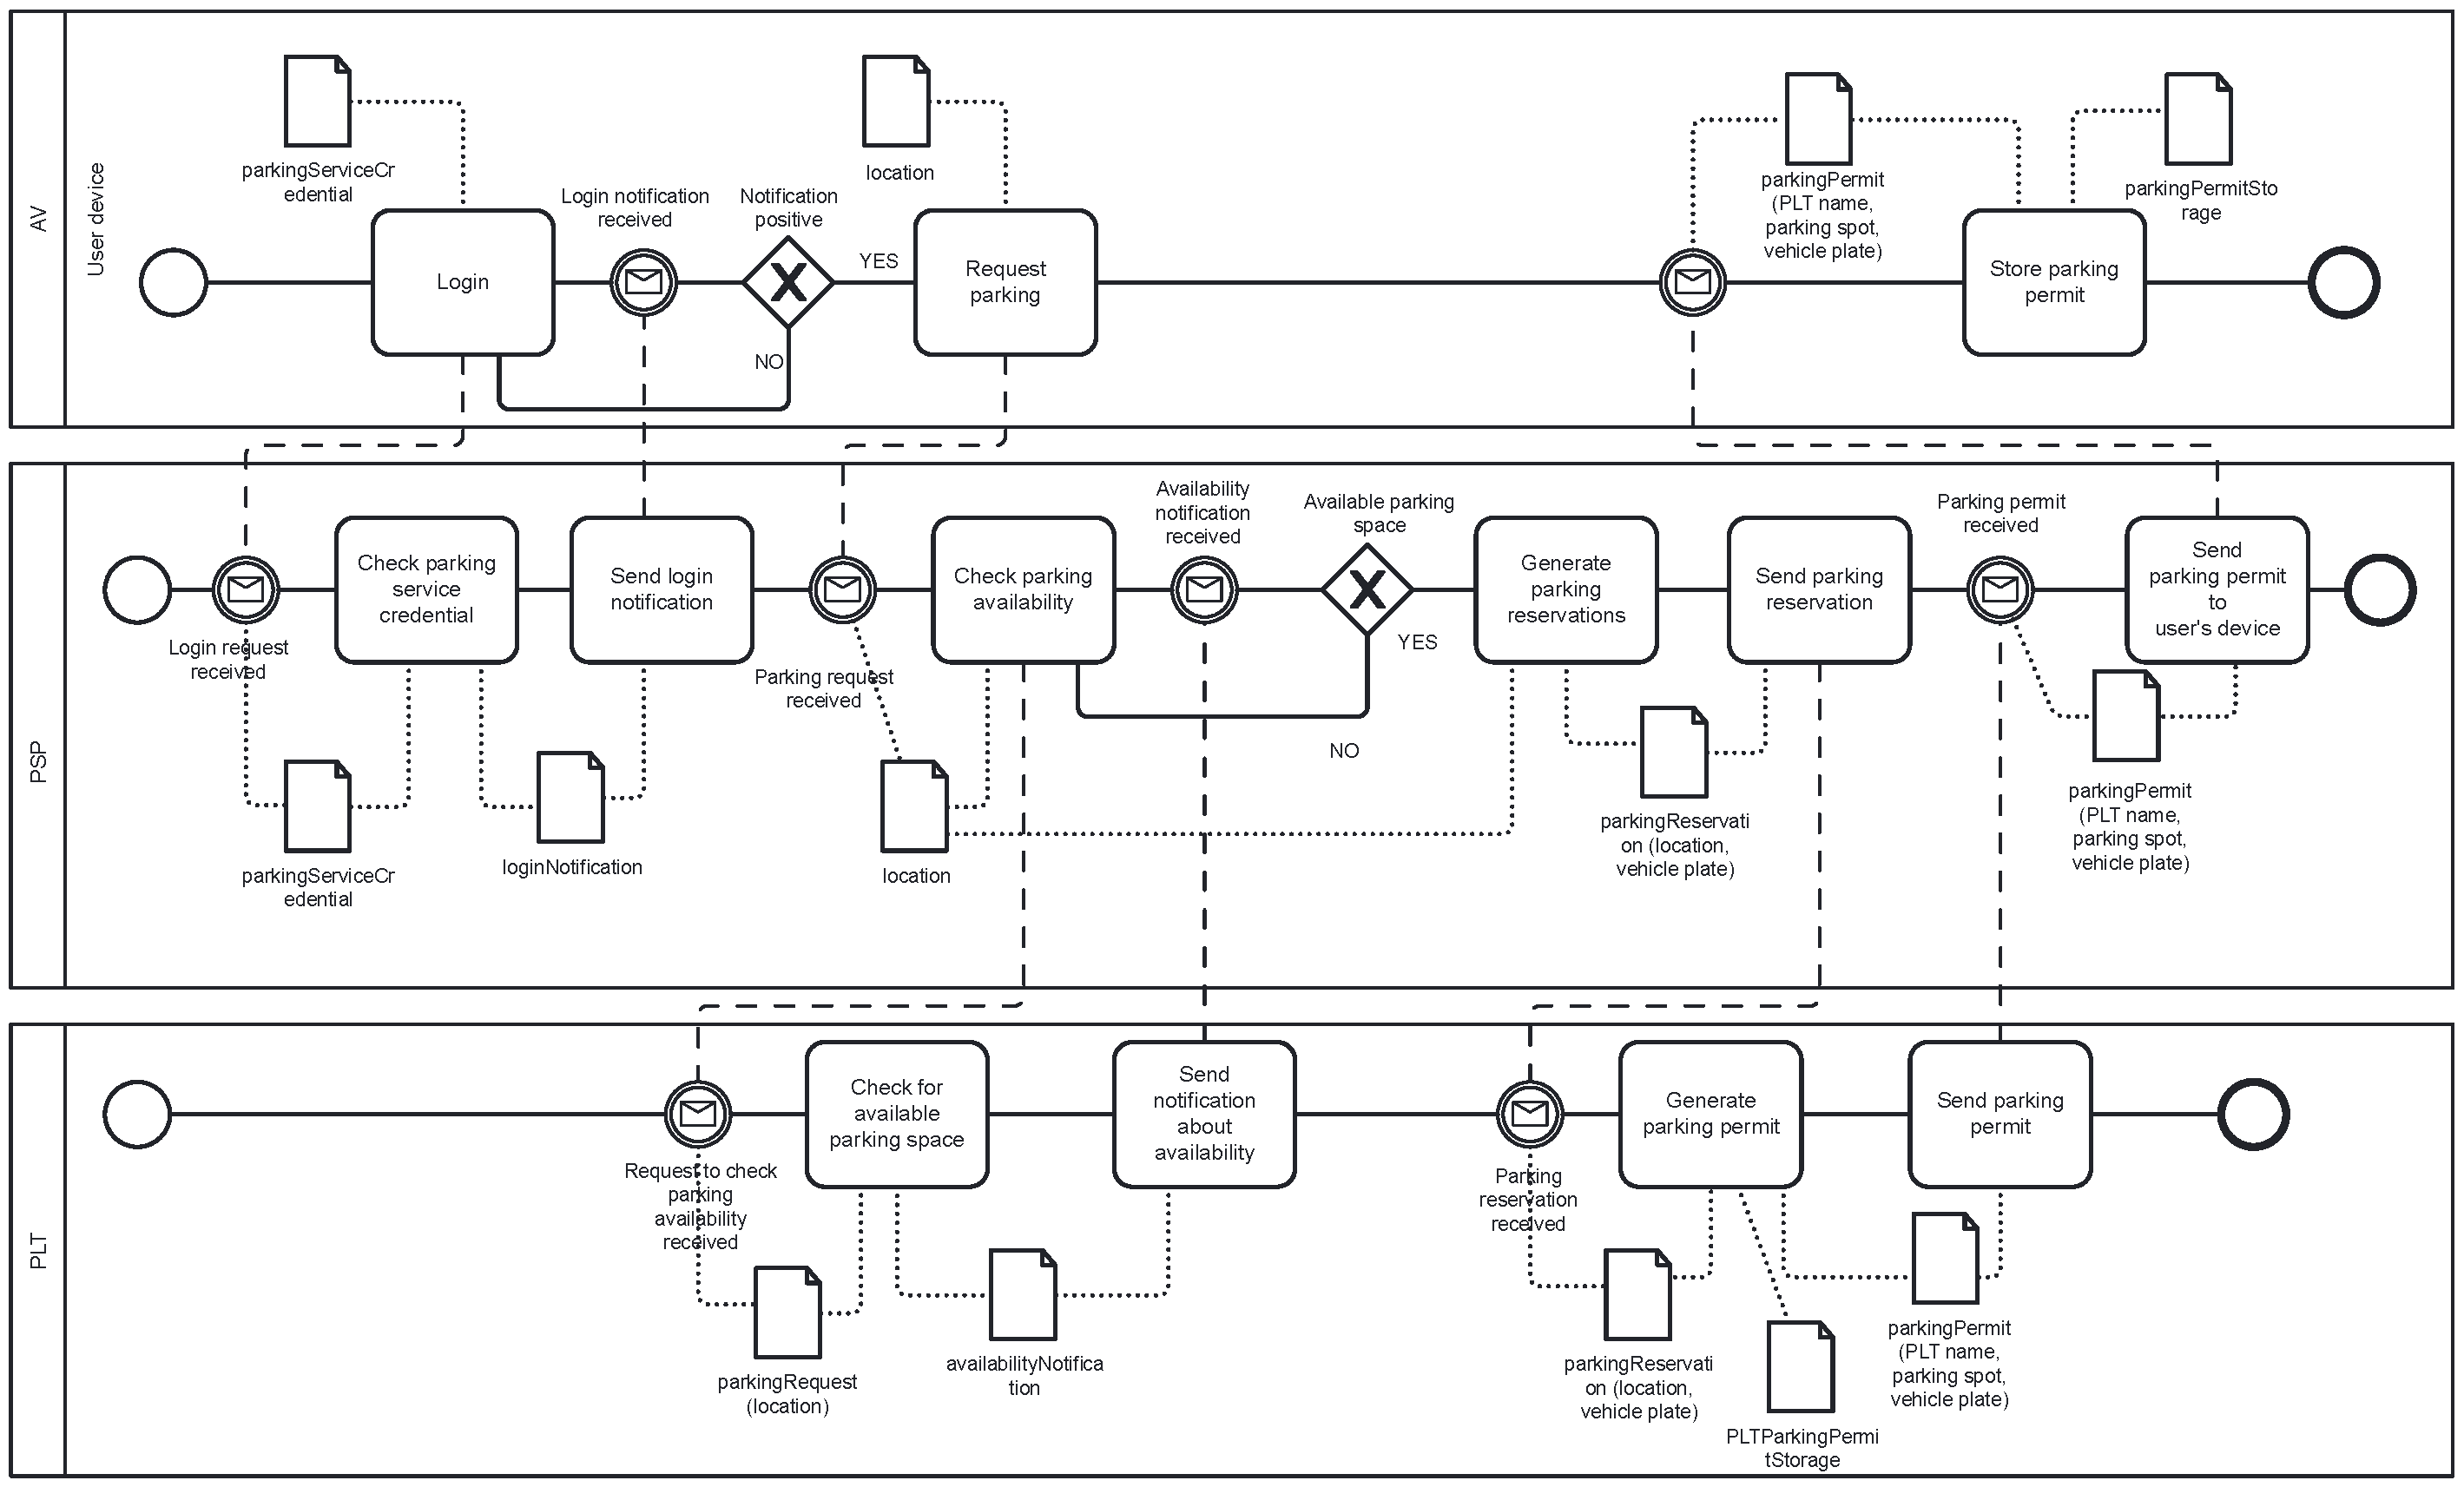
\includegraphics[width=\textwidth]{initial.pdf}
  \caption{Initial BPMN model (without GDPR annotations)}
  \label{fig:initial-model}
\end{center}
\end{figure}

The results of our analysis of the initial model with the DPO tool
(Figure~\ref{fig:initial-uml})~\cite{dpotool} revealed that several important
security measures are missing. These results align with our expectations because
of the aforementioned shortcomings, and the lack of GDPR annotations on the
model. Additionally, the analyses revealed the need for secure storage systems
to store the data and secure communication channels to transmit the data. All of
these measures are important to ensure compliance with privacy regulations and
to protect the privacy of personal data.


\begin{figure}[ht]
\begin{center}
  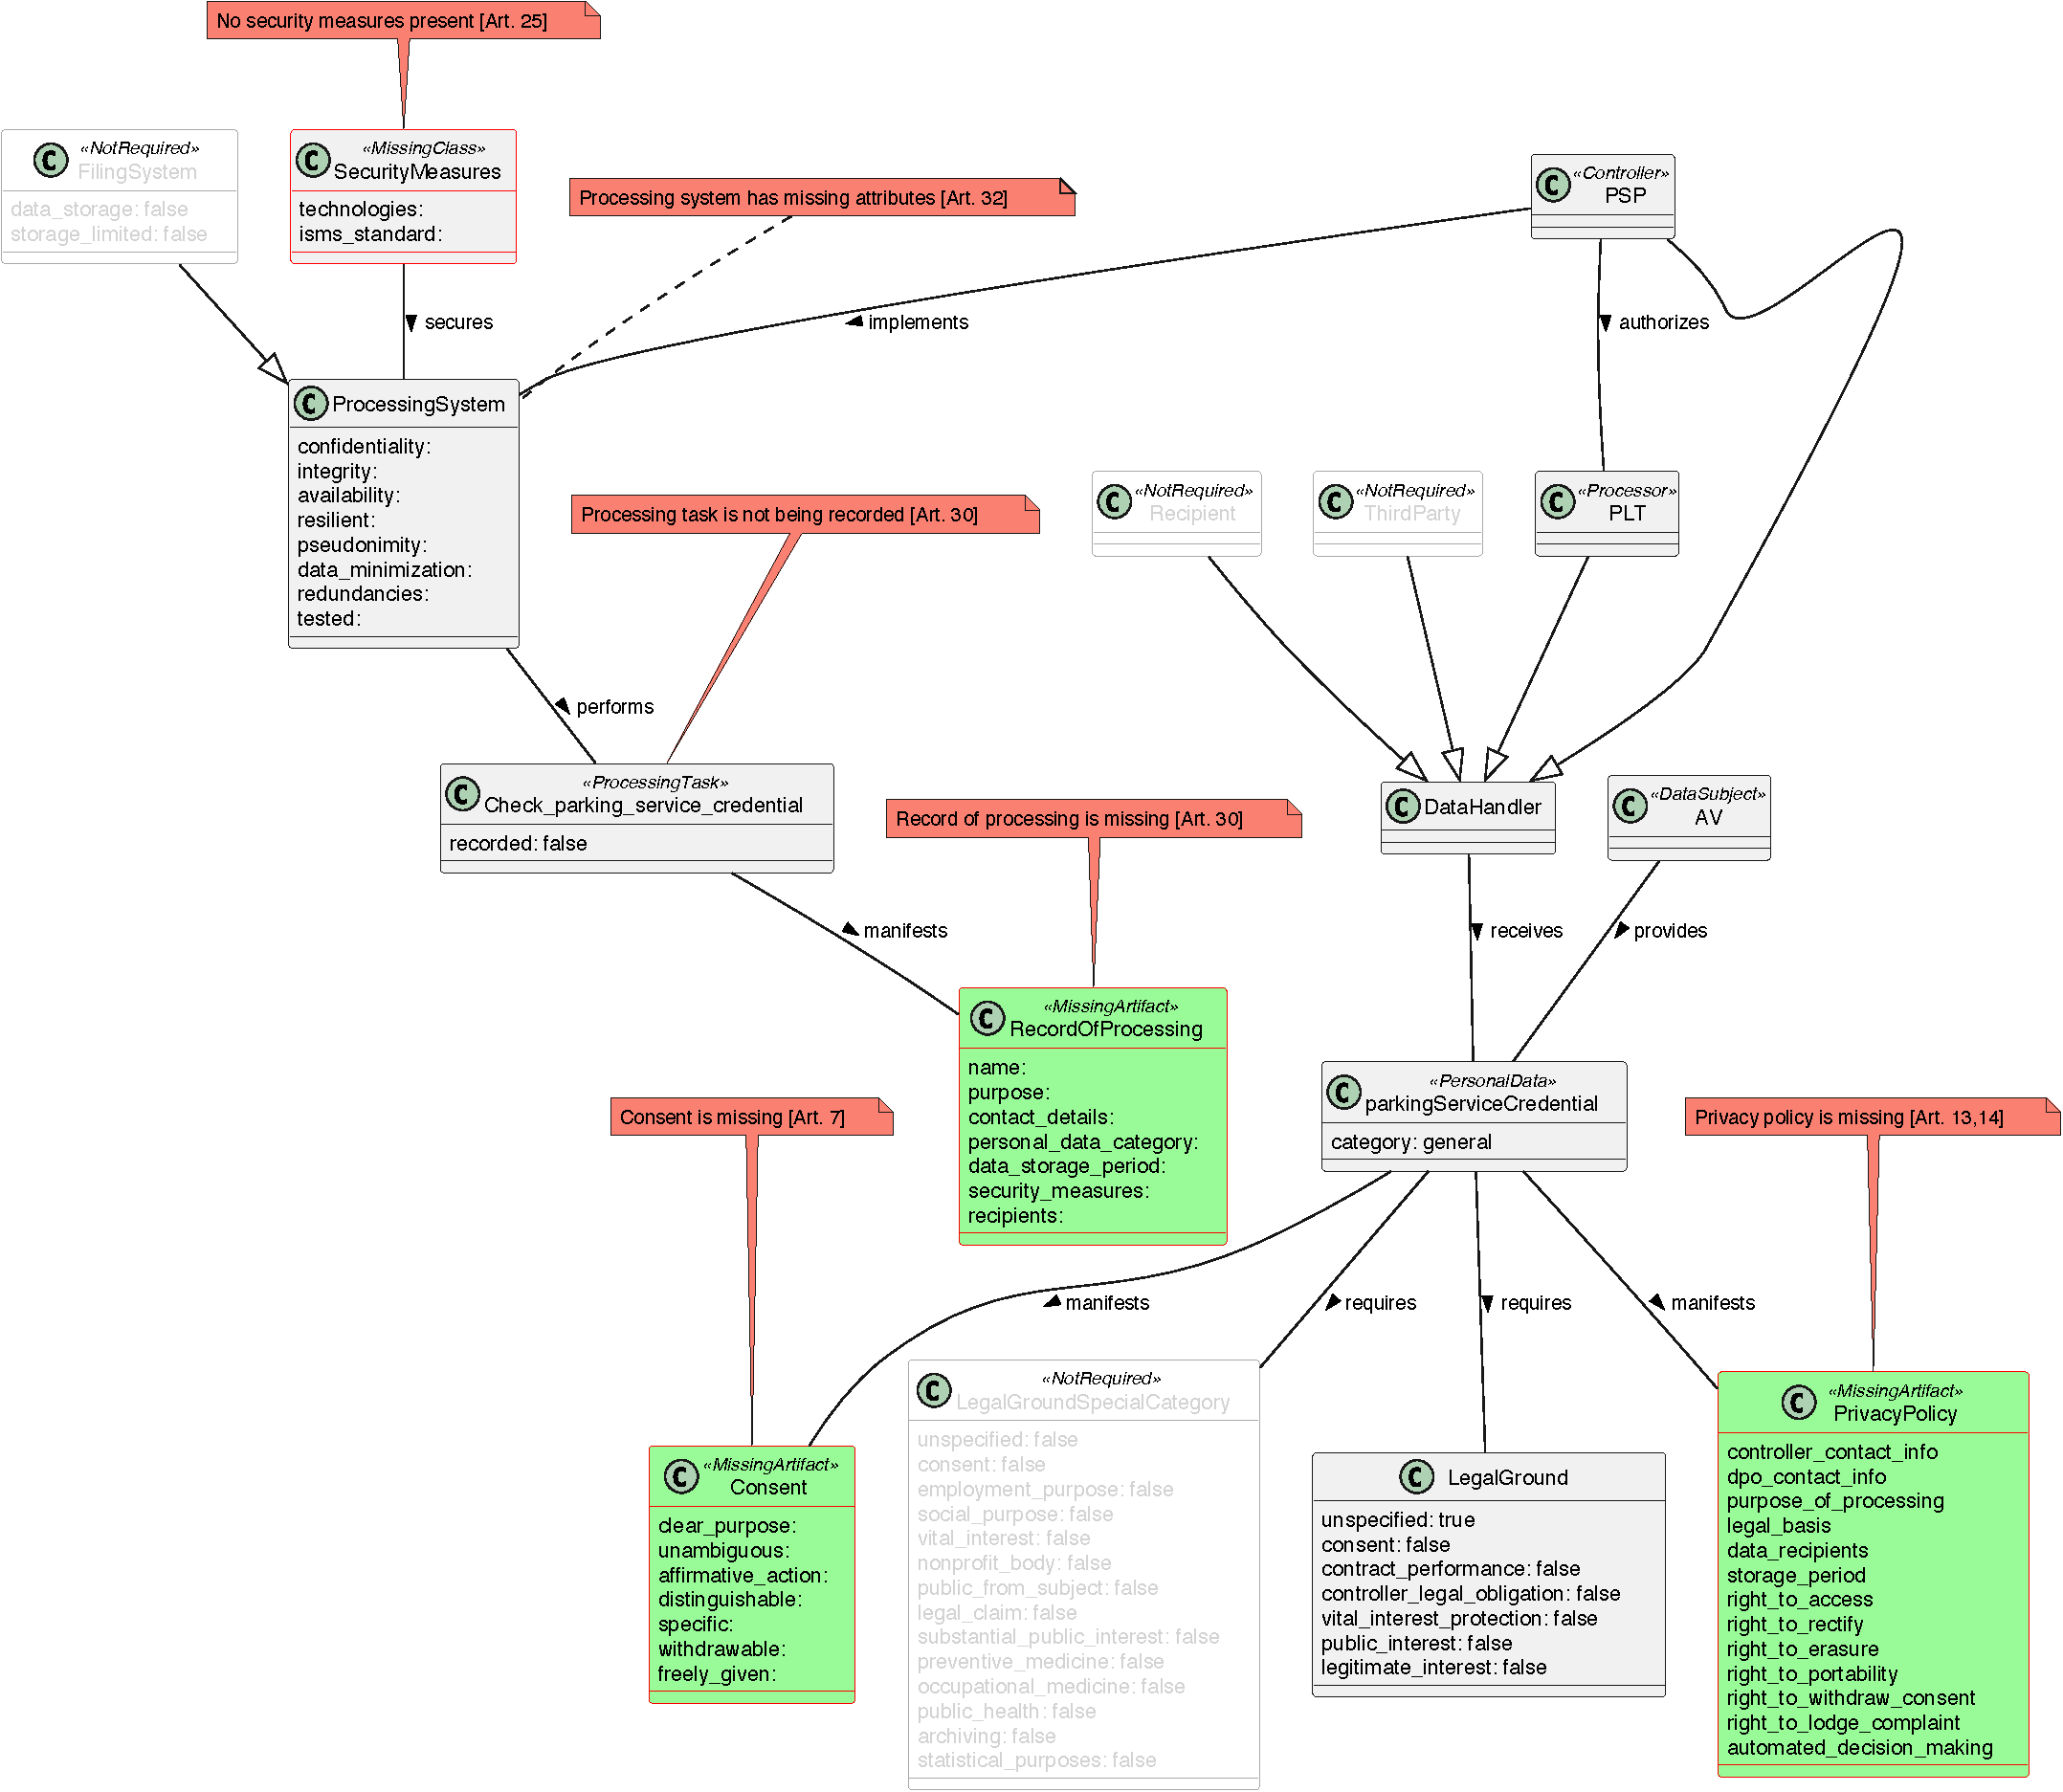
\includegraphics[width=\textwidth]{initial-uml.pdf}
  \caption{DPO tool analysis of the initial model}
  \label{fig:initial-uml}
\end{center}
\end{figure}

In summary, we identified the following aspects that are missing from the
scenario's model to make it GDPR compliant:
\begin{enumerate}
  \item no security measures present [Art. 25],
  \item the processing system has missing attributes [Art. 32],
  \item processing task is not being recorded [Art. 30],
  \item record of processing is missing [Art. 30],
  \item consent is missing [Art. 7],
  \item privacy policy is missing [Art. 13, 14].
\end{enumerate}

\section{Propose the privacy-by-design recommendations what should be done to
increase compliance and decrease data leakage}

To increase compliance and decrease data leakage, it is recommended to implement
a privacy-by-design approach that includes implementing technical and
organisational measures, regularly assessing data protection risks, and
verifying legal grounds for data
processing~\cite[110-111]{10.1007/978-3-030-58135-0_9}. In this case, we are
using the DPO tool which can offer guidance to achieve GDPR
compliance~\cite{dpotool}.

To achieve GDPR compliance, we annotated and made flow additions to the initial
model with the following ideas in mind:
\begin{enumerate}
  \item Prompt to introduce the \textbf{Privacy Policy} to the user (storage
  period, right to access, legal basis, \dots);
  \item Treat PSP as the \textbf{controller} and assign resulting obligations
  for data (confidentiality, integrity, availability, \dots);
  \item \textbf{Consent} needs to be taken from the user (clear purpose,
  unambiguous, affirmative action, \dots);
  \item Store a \textbf{record of document processing} with (purpose, contact
  details, data storage period, \dots).
\end{enumerate}

Figure~\ref{fig:improved-model} shows our improved and annotated model.

\begin{landscape}

\begin{figure}[ht]
\begin{center}
  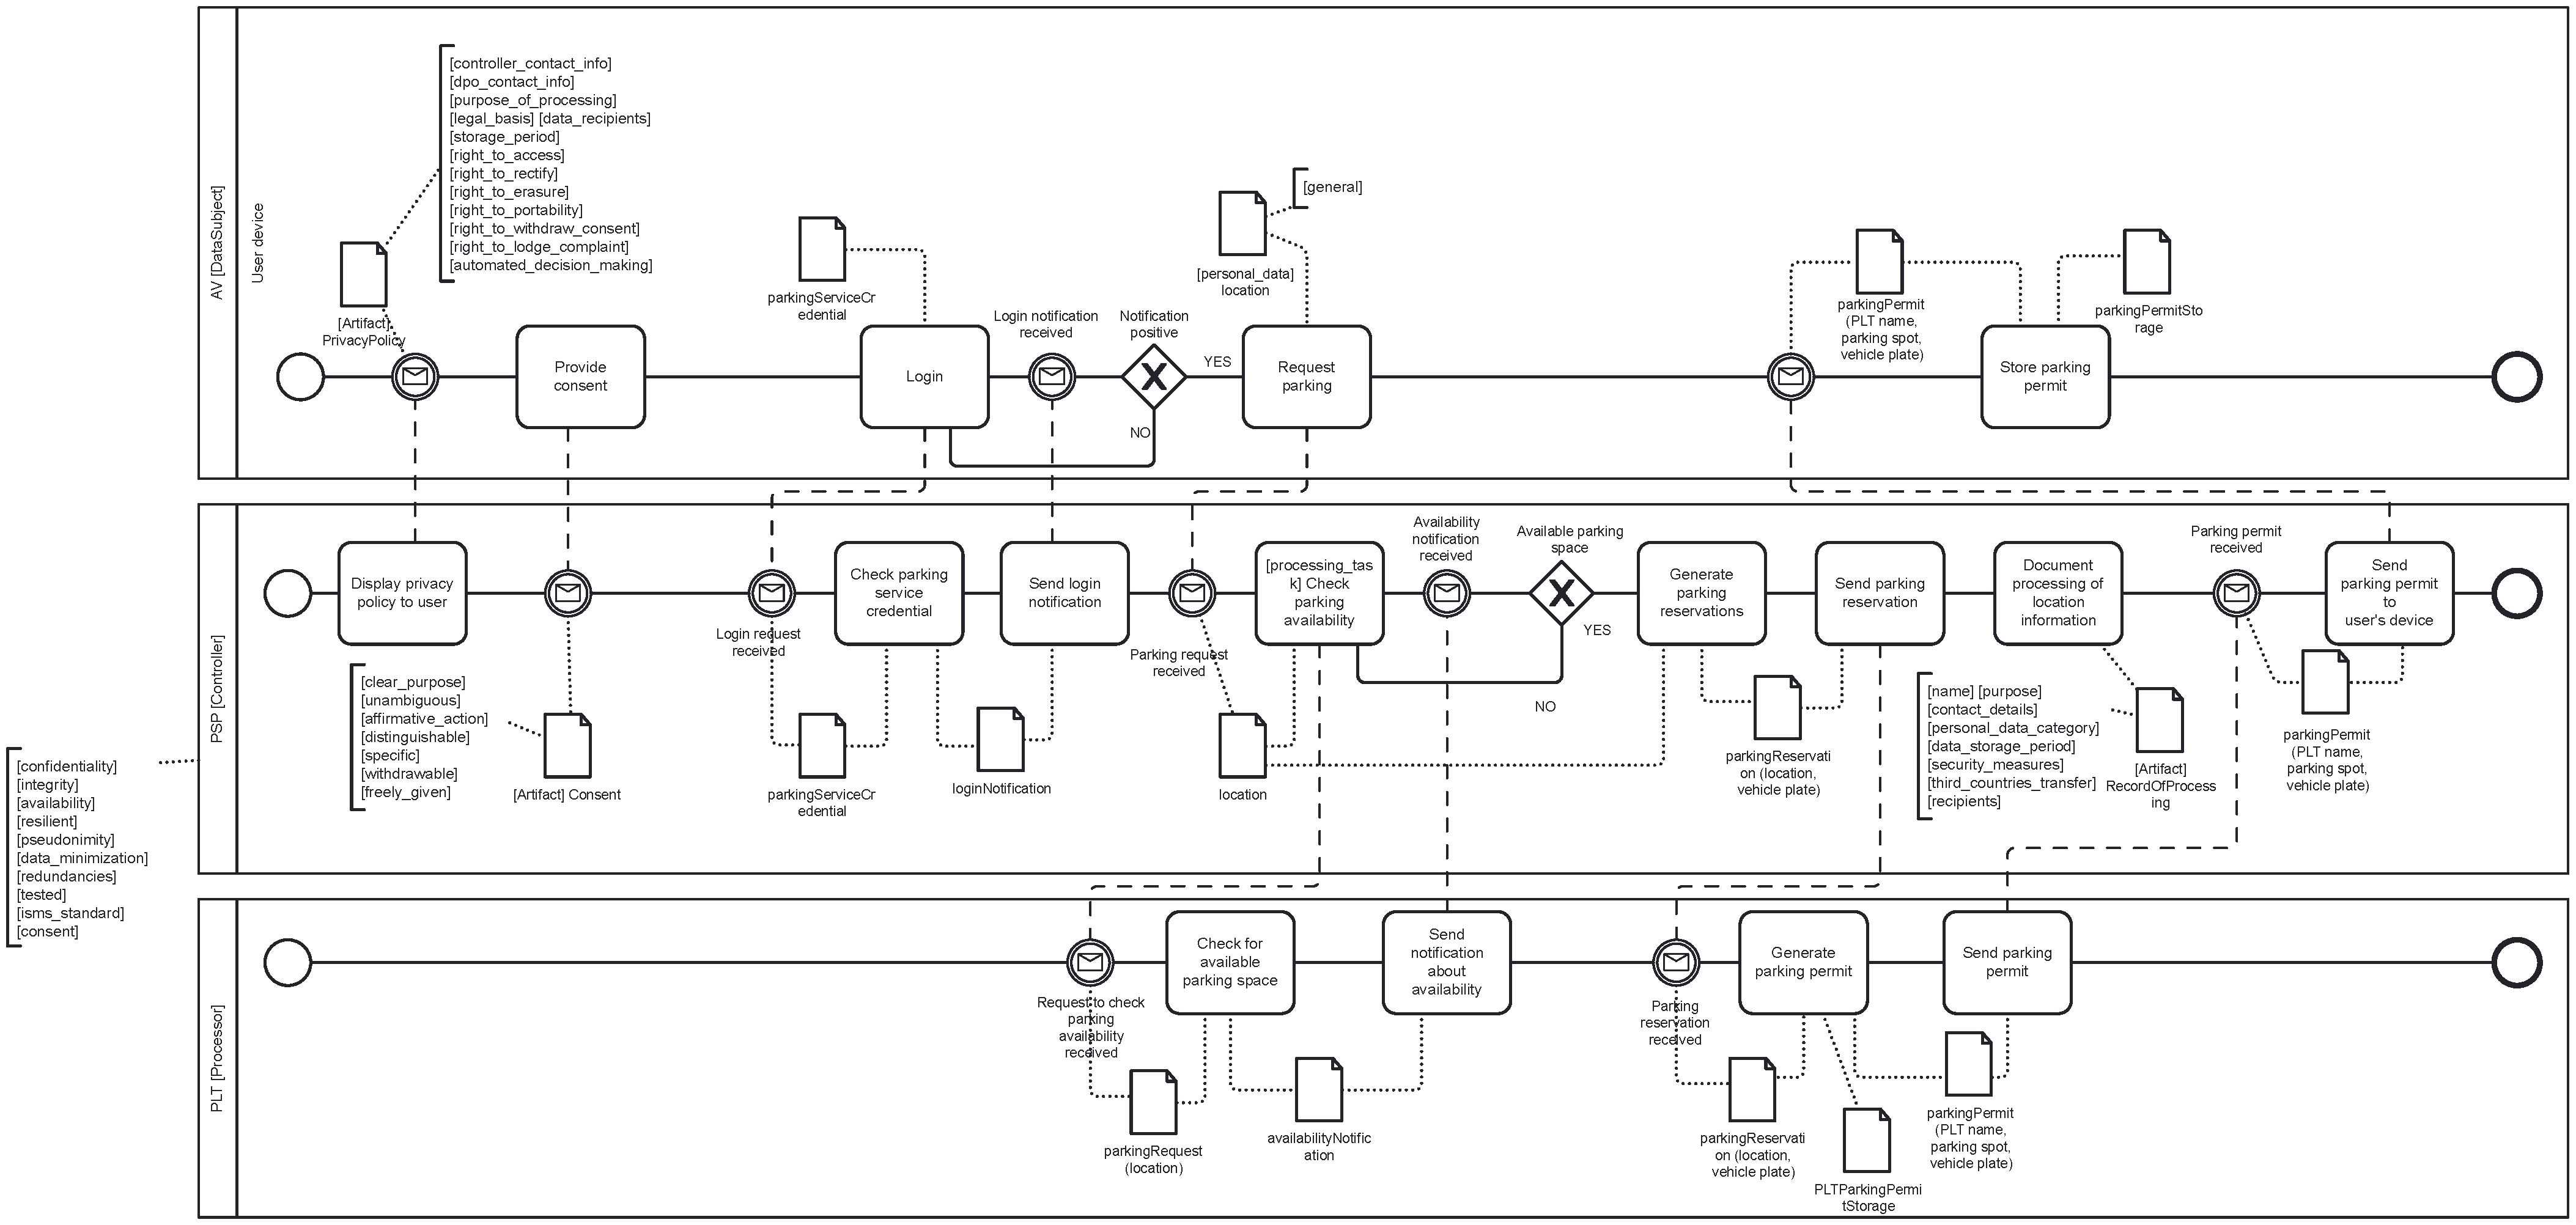
\includegraphics[height=\textwidth - 136pt]{improved.pdf}
  \caption{Improved BPMN model (with GDPR annotations)}
  \label{fig:improved-model}
\end{center}
\end{figure}

\end{landscape}

After performing a GDPR compliance analysis with the DPO tool on the revised
model, we obtained satisfactory results---all initial shortcomings were
addressed. Figure~\ref{fig:improved-uml} displays the result of the updated
evaluation.

\begin{figure}[!hb]
\begin{center}
  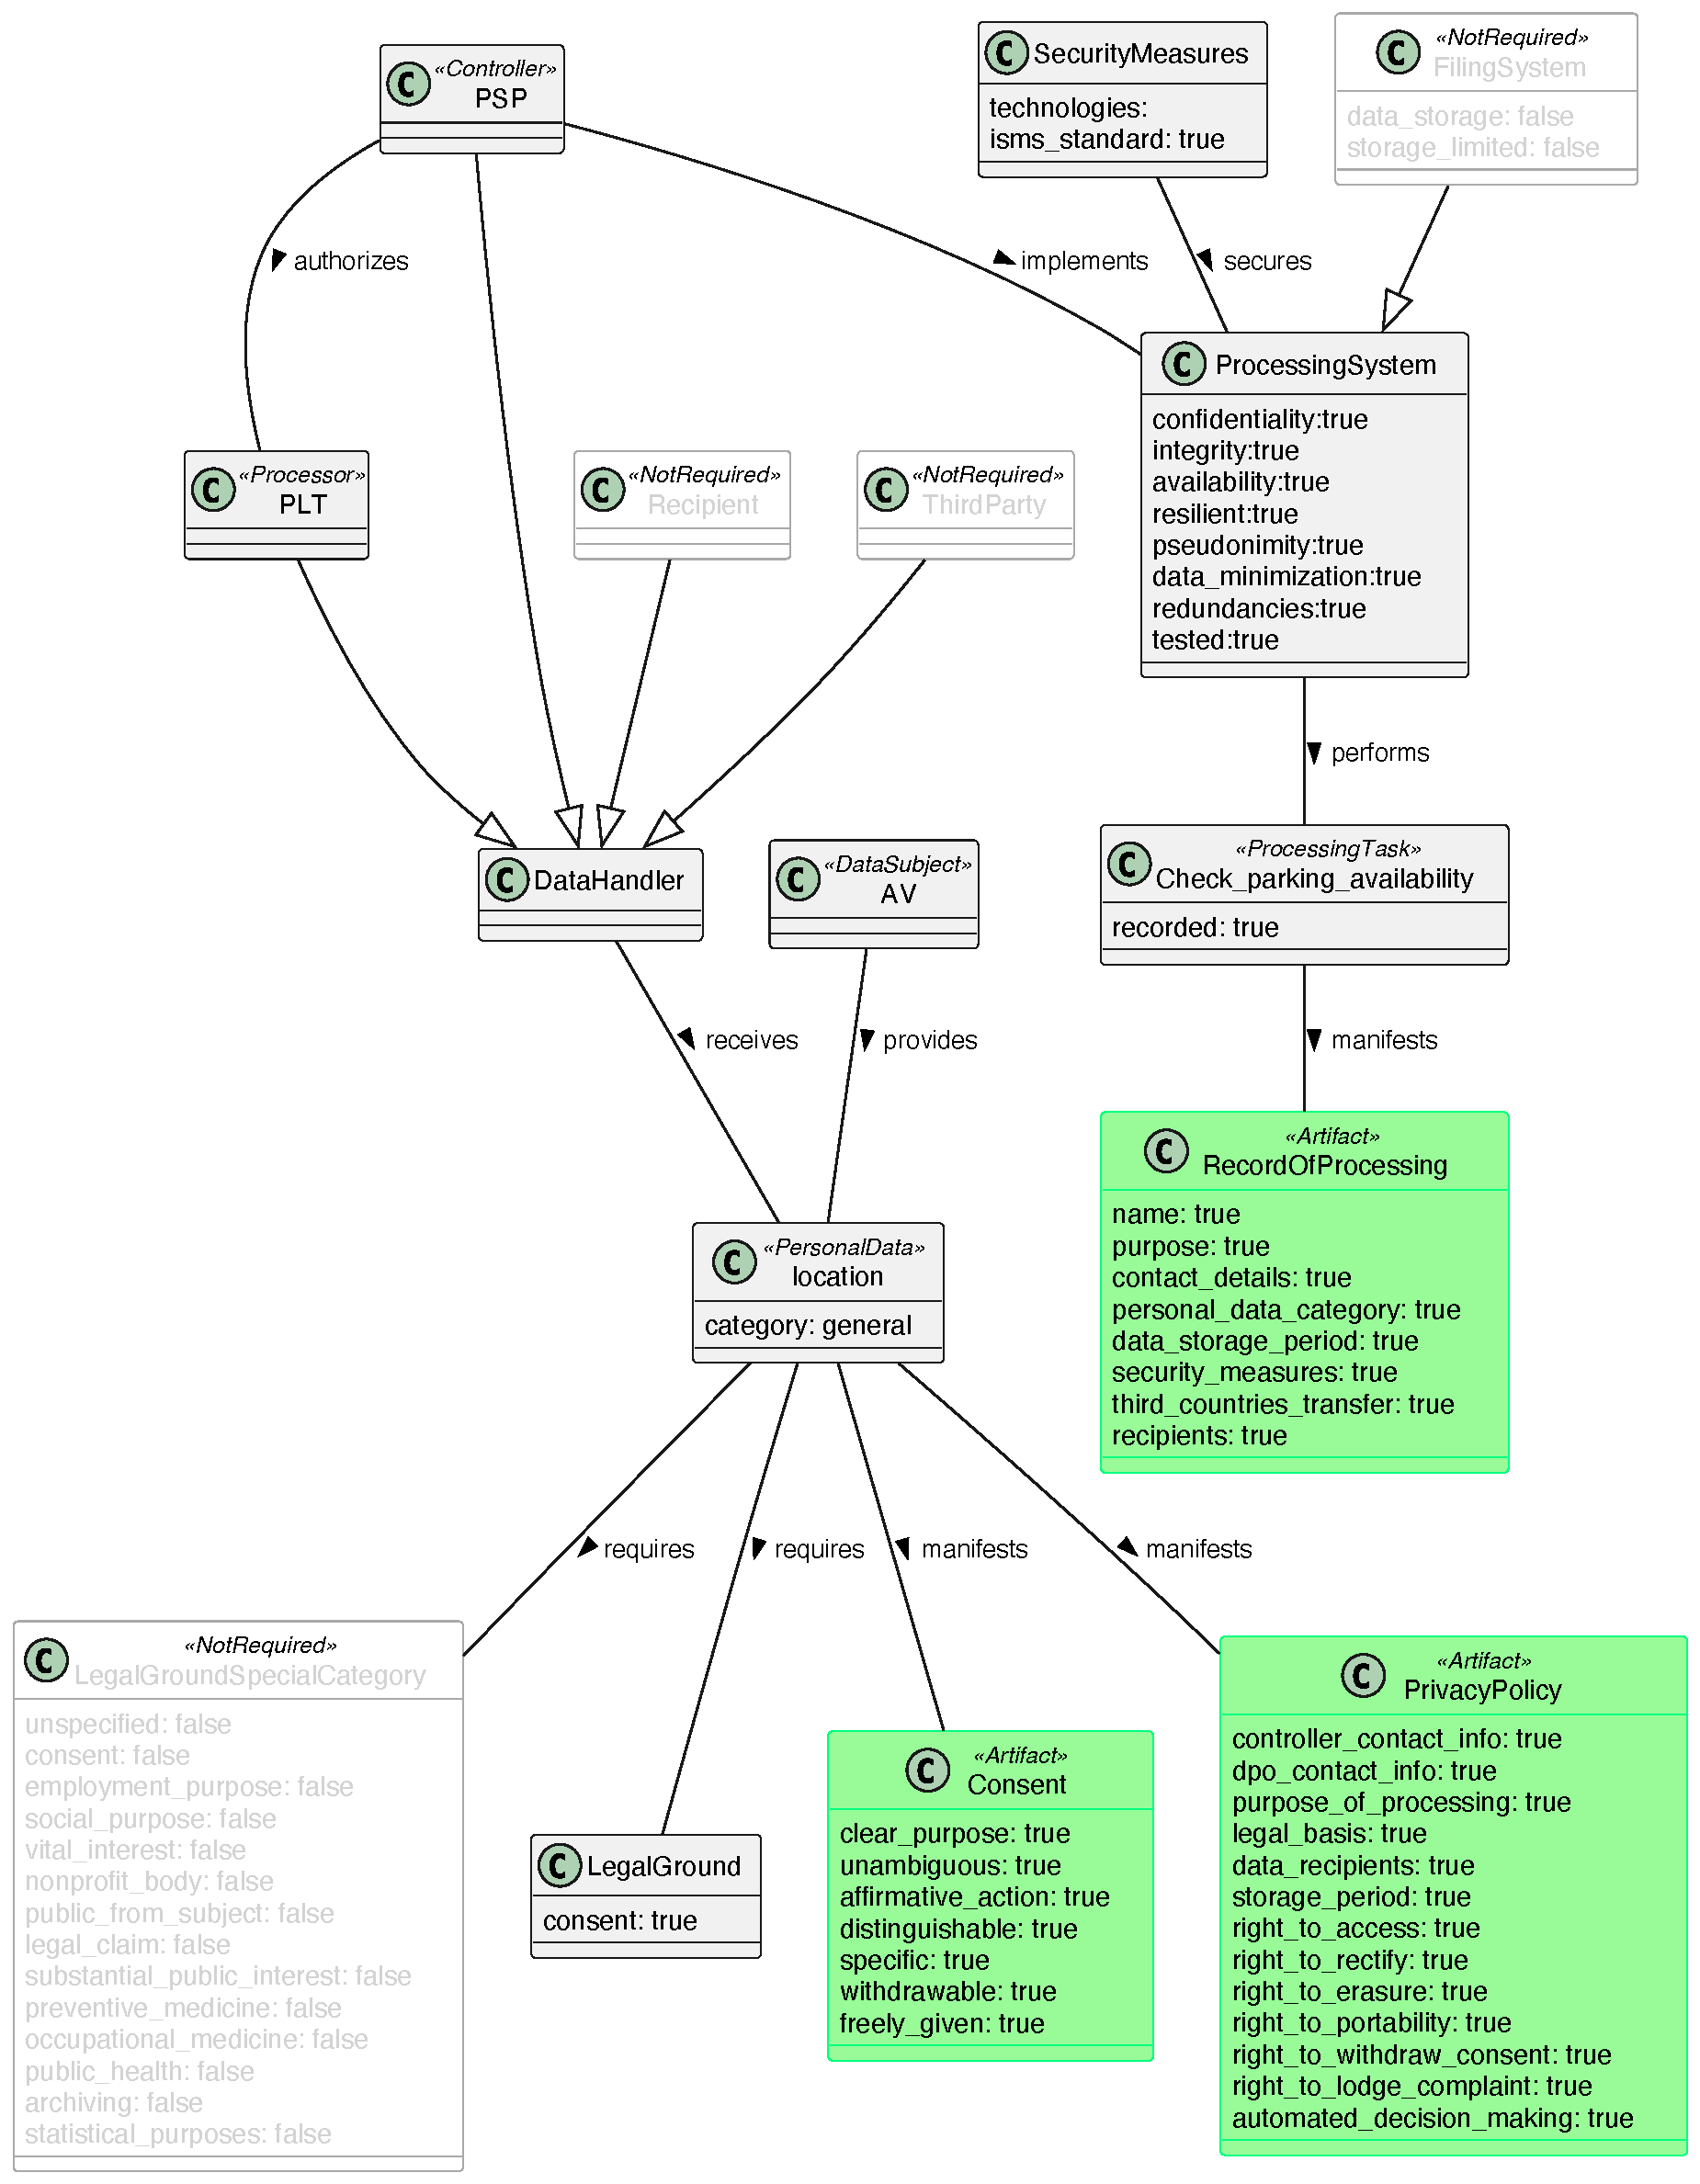
\includegraphics[width=\textwidth - 32pt]{improved-uml.pdf}
  \caption{DPO tool evaluation of the corrected model}
  \label{fig:improved-uml}
\end{center}
\end{figure}

\section{Apply the privacy-by-design principles using PE-BPMN}

We analysed our improved BPMN model (which is now GDPR compliant with added
annotations) and discovered several shortcomings---namely, the PSP and PLT can
put together the customer's identity and the location of their car, even when
this is not needed. For providing the parking service, it is sufficient if only
PLT learns of the parking location, and PSP of the user's identity. Moreover,
the PSP can read the parking permit information even though at this point the
PSP does not need to access these contents.

To help identify issues with the current process model, we used a tool called
Pleak \cite{pleaktool}. Pleak helps them to detect potential privacy risks by
identifying sensitive data, analysing data dependencies and performing
differentially private
computations~\cite[311-313]{10.1007/978-3-030-16722-6_18}. It also provides an
easy-to-use graphical interface for modellers to specify their business
processes and associated data flows~\cite{pleaktool}. The tool can quantify to
what extent a given output leaks information about the input, either in terms of
a sensitivity measure or in terms of the guessing advantage that an attacker
gains by having the output. Additionally, Pleak is a privacy-enhanced extension
of BPMN that enables the modelling of a wide variety of privacy-enhancing
technologies. This enables the analysis of privacy leakage risks and provides a
way to design processes that are more secure and compliant with privacy
regulations~\cite[1-3]{10.1007/s10009-021-00636-w}. Pleak is therefore a great
tool for helping to ensure compliance with data minimisation principles, such as
those outlined in the GDPR.

To protect the customer's data from parties not privy to certain details, we
opted for data encryption. The alternatives would have been secret sharing, data
splitting, or a hybrid approach. While the hybrid approach might offer some more
benefits in terms of privacy, using the encryption approach seemed to be the 
most rational in the current case, as there is no handling of any special type
of personal data (like health data, which might require higher levels of
protection). Adding third parties always comes with additional complexity, which
we did not wish to introduce here.

We note that our scheme assumes that a mechanism for key-exchange has been
agreed upon separately, and keys exchanged beforehand, for example during the
registration flow. The same assumption goes for the license plate information.
We did not add the key-exchange to the model as it is out of scope.

The analysis of the model depicted on Figure~\ref{fig:improved-model} provided
the following results:

\begin{center}
\begin{tabular}{ |c||c|c|c|c|c|c|c|c|c|c|c|c|c| } 
    \hline
    & 1 & 2 & 3 & 4 & 5 & 6 & 7 & 8 & 9 & 10 & 11 & 12 & 13\\ 
    \hline
    \hline
    PLT [Processor] & V & - & - & - & V & - & - & V & - & V & V & - & -\\
    \hline
    PSP [Controller] & - & V & V & - & - & V & V & V & - & - & V & V & -\\
    \hline
    User device & - & - & - & O & - & - & - & V & V & - & - & O & -\\
    \hline
    \hline
    Shared over & - & - & - &
    \multicolumn{1}{m{1.2em}|}{MF (V)} &
    \multicolumn{1}{m{1.2em}|}{MF (V)} &
    \multicolumn{1}{m{1.2em}|}{MF (V)} &
    \multicolumn{1}{m{1.2em}|}{MF (V)} &
    \multicolumn{1}{m{1.2em}|}{MF (V)} &
    - & - &
    \multicolumn{1}{m{1.2em}|}{MF (V)} &
    \multicolumn{1}{m{1.2em}|}{MF (V)} & -\\
    \hline
\end{tabular}
\\~\\
V = visible, H = hidden, O = owner, MF = MessageFlow, S = SecureChannel
\end{center}
where the header row numbers represent the following:
\begin{enumerate}
    \item PLTParkingPermitStorage
    \item {[Artifact]} Consent
    \item {[Artifact]} RecordOfProcessing
    \item {[personal\_data]} location
    \item availabilityNotification
    \item location
    \item loginNotification
    \item parkingPermit (PLT name, parking spot, vehicle plate)
    \item parkingPermitStorage
    \item parkingRequest (location)
    \item parkingReservation (location, vehicle plate)
    \item parkingServiceCredential
    \item {[Artifact]} PrivacyPolicy
\end{enumerate}

The results clearly show that the PSP can access the location of the user and
the parking permit, while PSP does not require access to those details. Using
encryption, we complemented our model by utilizing encryption and secure
communication channels. The complemented model is shown on
Figure~\ref{fig:pleak-model}.

\begin{landscape}

\begin{figure}[ht]
\begin{center}
    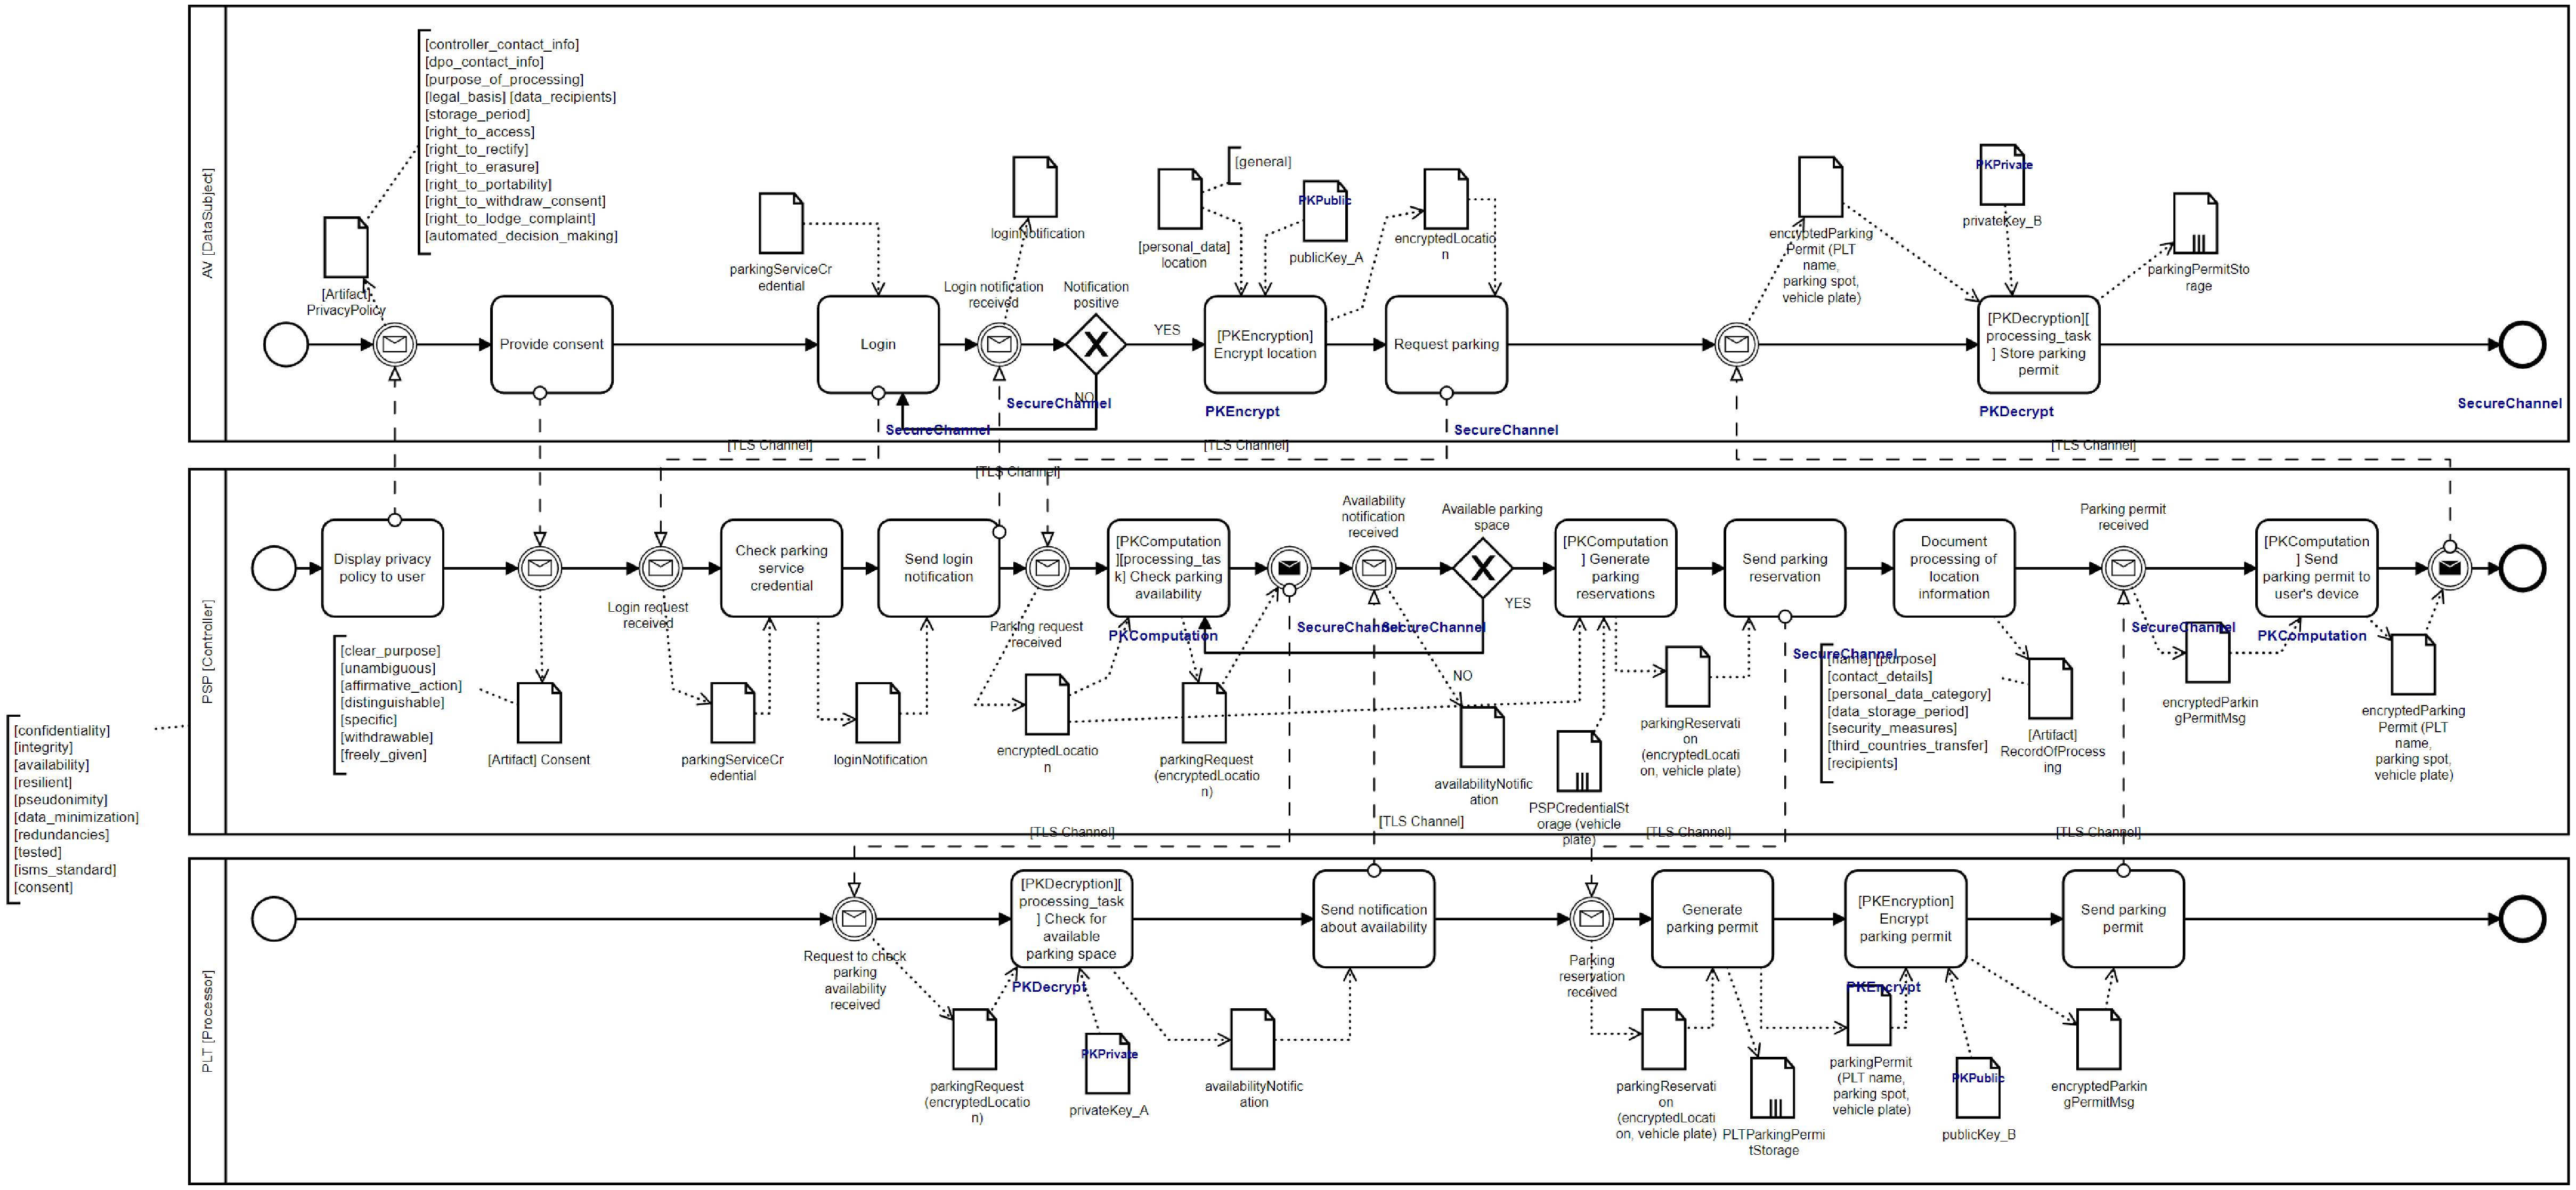
\includegraphics[height=\textwidth - 136pt]{pleak.pdf}
    \caption{PE-BPMN model}
    \label{fig:pleak-model}
\end{center}
\end{figure}

\end{landscape}

The analysis of our complemented model yields the following results:

\vspace{1em} % newline hack
\centerline{
\begin{tabular}{ |c||c|c|c|c|c|c|c|c|c|c|c|c|c|c|c|c| } 
    \hline
    & 1 & 2 & 3 & 4 & 5 & 6 & 7 & 8 & 9 & 10 & 11 & 12 & 13 & 14 & 15 & 16\\ 
    \hline
    \hline
    AV [DataSubject] & - & - & - & V & - & O & V & - & V & - & - & O & - & O &
    O & -\\
    \hline
    PLT [Processor] & V & - & - & - & - & - & - & V & - & V & V & - & O & - &
    - & O\\
    \hline
    PSP [Controller] & - & O & V & - & V & H & V & H & H & V & V & V & - & - &
    - & -\\
    \hline
    \hline
    Shared over & - & - & - & - & - & S & S & S & S & S & S & S & - & - & - &
    -\\
    \hline
\end{tabular}
}
\begin{center}
V = visible, H = hidden, O = owner, MF = MessageFlow, S = SecureChannel
\end{center}
where the header row numbers represent the following:
\begin{enumerate}
    \item PLTParkingPermitStorage
    \item PSPCredentialStorage (vehicle plate)
    \item {[Artifact]} Consent
    \item {[Artifact]} PrivacyPolicy
    \item {[Artifact]} RecordOfProcessing
    \item {[personal\_data]} location, encryptedLocation
    \item loginNotification
    \item encryptedParkingPermitMsg, parkingPermit(PLT name, parking spot,
    vehicle plate)
    \item encryptedParkingPermit (PLT name, parking spot, vehicle plate),
    parkingPermitStorage
    \item availabilityNotification, parkingRequest (encryptedLocation)
    \item parkingReservation (encryptedLocation, vehicle plate)
    \item parkingServiceCredential
    \item privateKey\_A
    \item privateKey\_B
    \item publicKey\_A
    \item publicKey\_B
\end{enumerate}


\newpage
\printbibliography
\addcontentsline{toc}{section}{\refname}

\end{document}
